\chapter{ANDROID FORENSICS}
\label{ch:forensics}
It is the goal of this thesis to outline a method of data confidentiality applicable to Android. The proposed method is only
meaningful in relation to data recovery techniques which are here collectively referred to as ``Android forensics.'' This chapter
gives an introduction to Android forensics.  The ``Android File Systems'' section discusses the YAFFS2 and ext4 file systems, which
are by far the most prevalent file systems on Android devices.  The ``Acquisition" section focuses on building and using the tools
necessary to acquire an ``image,'' of an Android partition, but also gives an overview of research regarding Android memory
acquisition. The analysis section discusses an example of how data can be extracted from an image once it has been acquired.  The
method of encryption proposed in Chapter \ref{ch:ecryptfs} is designed to defend against the specific methods of data
recovery touched on in this chapter.

\section{Android File Systems}

The YAFFS2 data presented here has been gathered from a Nexus One phone running Android version 2.3 (Gingerbread), and the
ext4 data has been gathered from a Nexus S phone running Android version 4.0.3 (Ice Cream Sandwich).  ``Nexus''
devices\footnote{Nexus One, Nexus S, and now Galaxy Nexus} are often favored by developers, as they provide a build of Android that
is as close as possible to the Android Open Source Project (hereafter AOSP). While Android is considered by many to be an open
mobile platform, not everything in Android is open source, meaning the source code for most, but not all, of Android has been
released for public inspection.  AOSP is that part of Android for which the source code has been released.  It includes the majority
of features in a consumer build of Android, but notably excludes many of the Google branded applications, such as Gmail and the
Android Market, as well as many device specific hardware drivers. The consumer builds for Nexus devices are not based on AOSP, but
they are much closer to AOSP than the builds shipped with other models, which often come loaded with third-party applications and
modifications to the underlying operating system.

Before diving into the details of Android file systems, it is important to understand how Android storage is laid out.  There are
typically two storage devices: an SD card\footnote{Often an actual, removable SD card is provided with the phone. Newer devices,
however, appear to be trending toward providing an emulated SD card from internal storage.} that is formatted with a FAT file
system, and an internal NAND\footnote{NAND is a type of non-volatile flash memory that is commonly used for file storage.} chip that
is formatted YAFFS2 or ext4, with newer models preferring ext4. Some device use other file systems on top
of NAND storage, such as the Samsung Galaxy S which uses a proprietary file system called \texttt{RFS}, but far and away
YAFFS2 and ext4 are the most common. The SD card is typically where large media files such as pictures and music
are stored. This paper, which is primarily concerned with application data, does not further discuss the SD card.

The number of partitions used by Android is device and version specific.  Android 2.3, for example, has up to six partitions,
excluding external storage: \texttt{boot}, \texttt{system}, \texttt{cache}, \texttt{userdata}, \texttt{recovery} and \texttt{misc}.
A Nexus S running Android 4.0, on the other hand, includes several additional partitions, such as \texttt{efs} and \texttt{radio}.
The \texttt{userdata} partition is the most interesting because it holds the data associated with each application.\footnote{
While this paper does not discuss partitions outside of \texttt{userdata}, from a privacy perspective it is important to realize
that sensitive information could still be leaked by other partitions, especially the SD card} To determine the file system layout
of an Android device:

\paragraph {1. Enable USB debugging} 
Figure \ref{fig:usbdebug} shows the \texttt{Development} menu for Android 2.3, where USB Debugging can be
enabled.  
\begin{figure}[htb]
\begin{center}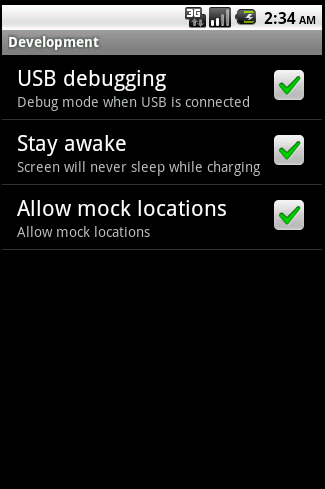
\includegraphics[scale=0.4]{usbdebug.png}\end{center}
\caption{Turning On USB Debugging}
\label{fig:usbdebug}
\end{figure}

\paragraph {2. Open an ADB shell}
Turning on USB debugging allows shell access to the device without entering a passcode. The shell is accessed with a utility called
the Android Debug Bridge (hereafter ADB), which is accessed by the command \texttt{adb}.  ADB is the primary means by which a
developer or forensic analyst will communicate with an Android device. The Android Software Development Kit (SDK) provides the
\texttt{adb} binary in \texttt{\$SDKPATH/platform-tools}.  ADB is the only practical way to obtain low-level access to an Android
device without physically removing the NAND chip.  When \texttt{adb} is first run, it starts a service that is then used to connect
to the Android device.  Once the \texttt{adb} service is started, a list of attached Android devices can be shown using the command
\texttt{adb devices}.

\paragraph {3. Run \texttt{cat /proc/mtd} and \texttt{mount}}
Opening a shell and displaying the contents of \texttt{/proc/mtd} results in output similar to Table \ref{tab:mtd}.  MTD is the
kernel driver in Linux that is responsible for providing the abstraction layer that is between file systems and ``Memory
Technology Devices'' (NAND memory). YAFFS2 is a consumer of the MTD interface, and \texttt{/proc/mtd} lists all of the active MTD
partitions. 
\begin{table}[htb]
\lstset{numbers=none}
\lstinputlisting{tables/procmtd.txt}
\caption{MTD Partition Layout of an Android Phone}
\label{tab:mtd}
\end{table}	

The layout in Table \ref{tab:mtd} was taken from a Nexus One running Android 2.3.  The first column is the device name which
corresponds to the device handle in \texttt{/dev/mtd}.  The second column shows the size of each partition in bytes.  The third
column gives the ``eraseblock'' size for the partition.  The eraseblock size determines the size of the smallest chunk of data that
can be erased on an MTD. In contrast to a more traditional block device such as a hard disk, the minimum I/O unit can vary for
different types of operations on NAND devices. Erasing is typically the most expensive operation for NAND flash. Each eraseblock
will consist of many NAND pages, which are the smallest unit of data the NAND device itself supports.  NAND pages are typically 2048
bytes, but the exact page size can be determined by looking at \texttt{dmesg} shortly after a device boots.  The fourth and final
column in \texttt{/proc/mtd} shows the friendly name of each partition.  

More recent Android devices use an Embedded MultiMediaCard (eMMC) interface. Rather than providing raw access to NAND memory, an
eMMC includes a controller that presents the NAND memory as a block device. The significance of raw NAND access will become more
clear when YAFFS2 is discussed in Section \ref{sec:yaffs2}.  When an Android device is using a file system such as ext4, which is
not designed for the limitations of NAND memory, an eMMC is used to provide wear-leveling, preventing the NAND chip from wearing
out.  The Nexus S actually has two storage chips: a straight NAND device and an eMMC. As show in Table \ref{tab:mount}, a Nexus S
does not use MTD devices for \texttt{system} or \texttt{userdata}. 
\begin{table}[htb]
\lstset{numbers=none}
\lstinputlisting{tables/mount.txt}
\caption{Nexus S Mounted File Systems}
\label{tab:mount}
\end{table}	

\subsection{YAFFS2} 
\label{sec:yaffs2}
YAFFS2 stands for Yet Another Flash File System, version 2. Many Android devices use YAFFS2 as the file system of choice for user
data that is not stored on an SD card.  YAFFS2 is very different from other file systems such as NTFS or FAT32.
YAFFS1,\footnote{The file system was actually just called YAFFS, but for the sake of clarity it is here referred to as YAFFS1.}
which preceded YAFFS2,  was the first file system specifically designed for NAND flash, and so its structure is optimized for the
specific requirements imposed by NAND flash.  Chief among these requirements is the limit on the number of overwrites performed.
NAND pages have a finite lifetime, and a file system that does not distribute wear will quickly wear out some pages.  The pages
storing the FAT in FAT32, for example, would quickly become corrupt without a hardware flash translation layer (FTL), as is used in
thumb drives to distribute wear more evenly.  YAFFS2 is designed to operate without a hardware FTL, which is good news for forensic
investigators, as it affords a software view into the flash device.  Overwriting NAND pages requires that those pages first be
erased, which in NAND incurs a heavy performance hit.  This leads to what is known as the ``write once" requirement, which is that
NAND pages should be written to only once unless it is absolutely necessary to overwrite them. The write once requirement has
influenced the design of YAFFS2 more than any other single factor.

YAFFS2 is known as a ``log-structured'' file system.  A log-structured file system does not reuse flash pages when a piece of data is
updated.  Rather, it simply writes the updated data to the next available location.  A monotonically increasing sequence number
keeps track of which data is most current, and the older versions of the same data are ignored.  This has dramatic forensic
implications, as it often means there are hundreds of copies of a given piece of data, even after it has been deleted.  YAFFS2 does
have a garbage collection routine that periodically erases old chunks in the background, but this routine appears to run
infrequently enough that forensic analysis of deleted data in YAFFS2 is still a valuable source of evidence \cite{naval}. 

YAFFS2 stores data in much the same way as its predecessor, YAFFS1.  Every piece of data written to a YAFFS1 based file system is
written in the form of a ``chunk," which is always the same size.  There are data chunks which hold the actual data in a file, and
there are object header chunks, which hold metadata about objects such as directories, files, and the like.  According to the
official YAFFS documentation \cite{howyaffsworks}, each chunk in YAFFS1
has the following information associated with it:

\begin{itemize}
	\item {\bf ObjectId}: Identifies which object the chunk belongs to.\
	\item {\bf ChunkId}: Identifies where in the file this chunk belongs. 
		A chunkId of zero signifies that this chunk contains an object header. 
		ChunkId 1 is the first chunk, ChunkId 2 the second, and so on.
	\item {\bf Deletion Marker}: Shows that this chunk is no longer in use.
	\item {\bf Byte count}: Number of bytes of data if this is a data chunk.
\end{itemize}

YAFFS1 relies on the Linux kernel's Memory Technology Device (MTD) driver to provide an interface to the actual NAND device.  The
Linux MTD presents the NAND device as a series of pages (usually 2kB), similar to blocks on a conventional hard disk.  Each page is
accompanied by 64 bytes known as the ``Out-of-band area," or OOB, which is partially used by the MTD itself and partially used by
the YAFFS1 file system. The MTD driver itself uses the OOB area to store error correction data, and additionally defines an area that
can be used by the file system for whatever purposes it chooses, called the OOBFREE area.  The layout of the OOB can be seen in the
\texttt{struct} in Table \ref{tab:oob}, taken from the Android source code. 

\begin{table}[htb]
\lstinputlisting{tables/oobstruct.c}
\caption{Out-of-Band Area (OOB) Structure}
\label{tab:oob}
\end{table}

The most important part of this \texttt{struct}, for our purposes, is the definition of the \texttt{oobfree} array.  The first element of the
\texttt{oobfree} array gives the offset into the area that is available for file system usage, and the second element determines the
size of that area.  There may be multiple arrays in \texttt{oobfree} leading to complex, non-contiguous free areas, but Android
appears to use one contiguous block.  This is not the standard layout used by Linux. Every file and directory within a YAFFS based
file system has an object header that is stored within this OOBFREE area. The object header describes the contents of the object,
which is stored in the data area of the chunk. This object header will include the object name, type, and length.  Notice that
because the object header contains the length, it must be written to every time the file length is changed.  Because a YAFFS based
file system writes sequentially, the new object header will be placed at the end of the object (with the same chunk id), and the old
object header will be marked deleted. 

YAFFS1 and YAFFS2 are actually remarkably simple compared to other file systems. To reiterate, the NAND device is divided into
pages, each with a small area for metadata (OOB).  The OOB defines what type of chunk that page belongs to, which chunk the page
belongs to, and in turn which object that chunk belongs to.  In YAFFS1 it also marks whether or not that chunk has been deleted.
Each object has a single object header and zero or more data chunks.  That's it.  Notice the conspicuous lack of any central
metadata location.  This makes the file system exceedingly simple, but at the price of \emph{scanning the OOB area of every page at
boot}.  There is no actual file system structure maintained on disk, just object headers and data chunks.  The file system layout is
determined at scan time and maintained in memory only. 

YAFFS2 is only slightly different from YAFFS1. The biggest change was the removal of the deletion marker, which was replaced with a
sequence number. Each time a page is written to it increases the sequence number by one, allowing pages with the same chunk id and
the same object id to be differentiated.  Whichever page has the largest sequence number is used, and the others are ignored.  Also,
in YAFFS2 the concept of a checkpoint was introduced to essentially store a snapshot of the data structures maintained in memory,
allowing for a faster boot.

\subsection{ext4}
The ext4 file system operates in a very different fashion than YAFFS2. While YAFFS2 was designed from the beginning to run on NAND
memory, ext4 was optimized for spinning disks. YAFFS2 went to great lengths to avoid overwriting NAND pages. In contrast, ext4
overwrites frequently, with no concern for the number of times a physical area of the disk is written to. Instead, ext4 is
interested in preventing the head on a hard disk from having to travel too far, and thereby mitigates the significant latency
introduced by mechanical movement. The fact that ext4 looks very different From YAFFS2 under the hood matters little to the rest of
the operating system, because the Linux kernel provides an abstraction layer called the virtual file system (hereafter VFS), which
sits on top of what is normally considered to be the ``real'' file system. VFS allows Linux based operating systems to switch
between different file systems with relative ease. The VFS interface presented to the rest of the system remains essentially
identical regardless of the file system in use, so the rest of the system need not worry about the particular file system being
used. Forensics practitioners, on the other hand, must be acutely aware of the file system in use. The ext4 file system is
enormously complex, but the basics are presented here.

The ext4 file system is an enhancement to the ext3 file system, which in turn was an enhancement to the
ext2 file system. The fundamental mechanics of ext2, ext3, and ext4 are very similar. Where the
operation of each is basically the same, the file system in question is referred to as ExtX, following the convention
introduced by Carrier \citeyear{carrier} in File System Forensic Analysis. 

The ``smallest addressable storage unit'' of a hard disk is a sector, and for an ExtX file system it is a block
\cite[Chapter 14]{carrier}. Typically the size of a sector is 512 bytes, and, by default, the Linux kernel treats all hard disks as
an array of 512 byte sectors \cite{linuxdrivers}.  A typical ExtX file system will use 4KiB blocks (eight sectors), but one
of the changes introduced by ext4 was support for block sizes of up to 64KiB. Data is read and written to the disk in
multiples of blocks, rather than bytes or bits. 

ExtX divides a disk into a series of block groups, the size of which is determined at the time of file system creation.  Each block
group contains a copy of the ``superblock.'' The superblock contains key metadata about the file system.  These copies can be used
for recovery should the primary superblock become corrupted.  Furthermore, because the metadata associated with a file is almost
always held within the same block group as the actual data for that file, block groups increase the performance of ExtX by
minimizing the amount of mechanical movement required of the hard disk. Additionally, the block group contains a ``group descriptor
table,'' which holds metadata about the layout of the block group itself, and an ``inode table,'' which holds information about the
files in the block group. In ext4 the block group layout has been modified with the introduction of ``flex block groups,'' which
centralize the metadata associated with a number of block groups, but this scalability improvement does not alter the basic ideas
behind block groups \cite{ext4implications}.

Each file has a piece of metadata associated with it called an inode, and the inodes for each block group are stored in the inode
table within the block group. All of the information about a file, excluding the filename and the actual contents of the file, are
stored in the inode. The inode structure includes, for example, the user ID (UID), the permissions mode, and pointers to the actual
data \cite[p.  457]{carrier}. Chapter \ref{ch:ecryptfs} uses the fact that each inode has a UID associated with it to derive an
encryption key for the contents of the file. Directories in ExtX are just a special type of file. The contents of a directory file
is a list of directory entries, which are data structures that contain the actual names of the files in the directory. In ext4 the
directory entries are stored in a hash tree structure by default, instead of a simple list which was the default for ext2 and ext3.
A directory entry contains a pointer to the inode for the file, enabling data retrieval based on the name of a file. 

When a file is deleted the directory entry is removed, the inode is deallocated, and the blocks associated with the file are freed,
but the actual data remains until, by chance, it is overwritten. The pointers in the inode that referenced the actual
data blocks are zeroed in ext3 and ext4, making it necessary to carve\footnote{Carving is the process of searching
for deleted files based on the structure of the files trying to be recovered. JPEG images, for example, can be identified because
they begin with the magic number FF D8.} for deleted files during recovery.  Most block allocation schemes do make an effort to
prevent file fragmentation, though, which increases the likelihood of being able to successfully carve for the file
\cite{ext4implications}. There has been some discussion of introducing secure delete functionality into ext4, but at the
time of writing it is not supported in most implementations \cite{ext4securedelete}.

There is an incredible amount of complexity necessarily being glossed over here, but the basics of ExtX have been covered.
A traditional spinning disk is addressed in sectors, and a series of sectors makes a block. ExtX contains a superblock,
which is just an area holding metadata about the file system. ExtX divides the disk into a series of block groups, and each
block group contains a copy of the superblock and metadata about the files within the group, including an inode table. Each file is
associated with an inode in the inode table, and the inode holds metadata about the file, including the location of the blocks
containing the file's data. Directories are just special files that hold filenames in directory entry structures, and a directory entry
points to the inode for the file. Deleting a file does not ensure that the contents of the file are gone, which is a fact frequently
used in forensics.

\section{Acquisition}
This section describes how the data on an Android device can be retrieved.  In a digital investigation, the primary source of
evidence is a copy of the target device's nonvolatile data.  Acquiring the nonvolatile data, be it from a conventional hard disk or
from NAND flash in a mobile device, is known as ``post-mortem'' acquisition, because the data is collected after the device has been
powered off.  Post-mortem acquisition is a well-established process, standing in contrast to live system acquisition, which is a
relatively new and quickly evolving process, even for desktop and laptop computers.  Forensic acquisition of mobile devices follows
the same principles as more traditional forensic acquisitions, but the tools, techniques, and limitations can be very different. The
process of acquiring a system, whether it be a desktop or a mobile device, is of primary interest to digital investigators and
incident responders. They typically adhere to procedures and practices that create ``forensically-sound'' duplicates.  According to
Craig Ball, 
\begin{quote}
“A ‘forensically-sound’ duplicate of a drive is, first and foremost, one created by a method which does not, in any way, alter any
data on the drive being duplicated.  Second, a forensically-sound duplicate must contain a copy of every bit, byte and sector of the
source drive, including unallocated ‘empty’ space and slack space, precisely as such data appears on the source drive relative to
the other data on the drive. 
\cite{ball}
\end{quote}
The forensically-sound duplicate outlined by Ball is usually acquired by physically removing the hard disk from the target system.
The hard disk is then attached to a write blocking device and copied using one of many possible acquisition utilities, creating an
``image" of the drive. For analysts of average means, creating a forensically-sound duplicate of an Android device can be
challenging. The operating system itself and the majority of forensic artifacts (with the exception of pictures, media files, and
some application data) are stored on internal flash memory.  Removing the flash memory and attaching it to a write blocker is, while
theoretically possible, beyond the reach of most forensics labs due to the sophisticated electronics work involved.  The NAND memory in
many devices could conceivably be accessed either through the JTAG\footnote{JTAG stands for ``Joint Test Action Group.'' JTAG test
access ports are available on most devices.  They are used to access the CPU to perform debugging operations, and in certain
situations can be used to bypass security mechanisms or directly access NAND storage.} ports in the device, or by physically
removing the chip.  Either method would require significant electronics work and further reconstruction of the low-level NAND
layout. Directly accessing the NAND flash is a last resort, but it may be the only possibility on a properly locked device
\cite{chipoff}.  Further challenges are presented by the inability of standard users to perform the low-level operations necessary
to forensically acquire a device, as the Android security model does not usually provide root access.  Additionally, flash memory
stores metadata in a fashion that is not taken into account by traditional forensic acquisition methods.  What the average forensic
analyst ends up with, then, is only an approximation of a forensically-sound duplicate of an Android device. 

\subsection{A Basic Android Acquisition}

In broad strokes, the acquisition of an Android device is not much different than the acquisition of a desktop computer. 
The device must be seized, and an image of the device must be created that is as forensically sound as possible.  There are,
however, several Android specific details that must be addressed.  What follows is an overview of the steps necessary for acquiring
an Android device, partially drawn from Andrew Hoog's book \emph{Android Forensics} \cite{hoog}.

\paragraph{Step zero: build tools and document procedures}
Perhaps it goes without saying, but it is imperative that the acquisition tools and procedures be developed \emph{prior} to
acquisition.  If the device is using YAFFS2 as the file system (the majority of devices at the time of writing), \texttt{nanddump}
should  be used.  The process of building \texttt{nanddump} from source is described later in the chapter.  The Android Debug
Bridge, provided with the Android SDK as a means of communicating with the device over a USB cable, should be installed and tested. 

\paragraph{Step one: initial seizure}
The target device must first be secured in the analyst's possession, physically and electronically.  If the device is unlocked at
the time of seizure, it should be immediately determined if a passcode or disk encryption is enabled. If either protection is
enabled, as much data as possible should be acquired while the device is running and unlocked.  If the device is encrypted and
already off, then more creative methods will need to be employed (see chapter \ref{ch:fde}).  The version of Android should be
retrieved from the settings menu prior to shutting the device down and USB debugging should be enabled if possible.  Unless a
logical analysis is going to be performed, or the device is encrypted, it should be powered off.  Finally, the device should be
isolated from the network, either by turning it off or placing it in a Faraday bag.

\paragraph{Step two: unlock the device}
If the device is locked, the password will need to be guessed or bypassed, either through brute-force, a smudge attack, or some
other means.  A smudge attack involves reading the residual oil patterns off of a touch screen in order to determine the unlock
pattern or PIN \cite{smudge}. The SIM card should be removed and analyzed separately, though SIM cards used in Android devices do
not make particularly interesting pieces of evidence, as the majority of data is stored on the device itself.

\paragraph{Step three: image SD card}
 If removable, the SD card should also be removed and analyzed separately (in the same fashion as a thumb drive). A zeroed SD card
should be placed in the device for storing NAND images. If the SD card is not removable, as in the case of the Nexus S which uses
eMMC to provide USB mass storage, then it can be imaged through \texttt{adb} \cite[pp. 211-218]{hoog}.
 
\paragraph{Step four: root the device}
Unless root access has previously been enabled on a device, some sort of privilege escalation is generally required before an image
of the device can be taken. The fact that exploitation is regularly involved during the process of acquisition startles many, yet it
is often the only way to obtain access. By default, Android does not provide root access even to the device owner.  A substantial
amount of research should be done about the device before attempting to obtain root access, since an incorrectly executed attack can
lead to inadvertent data loss. Any analyst of modest means (i.e. without an exploit development team) is at the mercy of the
security and hobbyist communities for rooting methods. If the device cannot be rooted, then an image of the device cannot be taken
and a logical acquisition will have to suffice. A logical acquisition consists of manually inspecting the device from the user
interface, or installing an application that will systematically read unsecured data.

\paragraph{Step five: acquire an image of \texttt{userdata}} An image of each partition on the device can be acquired with either
\texttt{dd} for ext4 or \texttt{nanddump} for YAFFS2.  These images should be stored on the sterile SD card that was previously
inserted into the device.  

One of the most popular tools for acquiring an image of a conventional (spinning disk) hard drive is
\texttt{dd}, which reads raw data, block by block, from one location and writes it to another, which, when the disk is offline, is
sufficient to acquire a forensically valid image of the device.  Any Nexus device should already come with a functional copy of
\texttt{dd} that can be used to copy an ext4 partition.  Table \ref{tab:dd} shows the process of acquiring an \texttt{ext4 userdata}
partition from a Nexus S phone.  After the image has been transferred from the SD card to the analyst's machine, it can be mounted
for perusal or carved for deleted files.  

\begin{table}[htb]
\lstset{numbers=none}
\lstinputlisting{tables/dd.txt}
\caption{Copying an ext4 Partition with \texttt{dd}}
\label{tab:dd}
\end{table}

Acquiring an image of a YAFFS2 file system presents a distinct challenge.  
Unfortunately, \texttt{dd} is not sufficient for YAFFS2 devices, as it operates above the MTD layer, and YAFFS2
makes use of the OOB free area. Android images that are acquired by a utility that is not flash-aware lose a lot of metadata. In the
case of YAFFS2, it is difficult to discern between active and stale areas of the file system without the metadata stored in
the OOB free area. Section \ref{sec:nanddump} discusses the use of \texttt{nanddump} to acquire an image that does contain the OOB
area.

\subsection{Nanddump}
\label{sec:nanddump}
Hoog's book \cite{hoog} provides an excellent primer on how Android forensics is performed.  Unfortunately, a great number of
implementation details are glossed over in favor of describing opaque forensic tools, such as Hoog's own AFLogical/AFPhysical tools,
or Cellebrite's more well-known UFED. These tools are only available to the law enforcement community, limiting their academic
value. The tool used here for acquiring Android images is \texttt{nanddump}. Hoog's tool set makes use of the same tool.

Unlike \texttt{dd}, \texttt{nanddump} does acquire the OOB area in addition to the data portion of a NAND device.  In Ubuntu,
\texttt{nanddump} is provided by the \texttt{mtd-utils} package.  The binary that comes with the \texttt{mtd-utils} package is not
compiled for the ARM processor, however, and so it must be cross-compiled before it can be used on an Android device.  The following
set of steps can be used to create an ARM \texttt{nanddump} binary.  The procedure was tested on Ubuntu 10.04.3 amd64, using version
20090606 of the \texttt{mtd-utils} source package, and version 2011.03 of the CodeSourcery G++ Lite Edition for ARM (now branded
Mentor Graphics).  These steps are an adaptation of a guide provided at elinux.org \cite{compilingmtd}.

Assuming \texttt{nanddump} is being built on a 64-bit machine, 32-bit runtime libraries must be installed.  In Debian-based
distributions, these are provided by the \texttt{ia32-libs} package.  After installing the necessary libraries, CodeSourcery G++ Lite
is easy to get up and running by simply downloading the tools and extracting them to a convenient location.\footnote{Download available
from
\url{https://sourcery.mentor.com/sgpp/lite/arm/portal/package8739/public/arm-none-linux-gnueabi/arm-2011.03-41-arm-none-linux-gnueabi-i686-pc-linux-gnu.tar.bz2}
at the time of writing.} It does not matter where the build suite is installed, but the \texttt{bin} subfolder in that directory
must be part of the \texttt{PATH} environment variable.

Once CodeSourcery is installed, one must obtain the source code for nanddump and then cross-compile compile it with the CodeSourcery
\texttt{gcc}.  The source code from \texttt{nanddump} is provided by the \texttt{mtd-utils} source package and can be retrieved
using \texttt{apt-get source} on a Debian based system.  The source code can also be obtained from the project homepage at
\url{www.linux-mtd.infradead.org}.  The \texttt{mtd-utils} package includes the source code for a number of other utilities that
are not needed for \texttt{nanddump} to operate.  Since building the entire \texttt{mtd-utils} package is mildly complicated, the
easiest and recommended route is to copy out \texttt{nanddump.c} and the \texttt{include} directory, and build \texttt{nanddump}
separately.  An example shell script that performs the entire process can be seen in Table \ref{tab:nanddump}.  Because the Android
build system is not being used, it is imperative that \texttt{nanddump} is statically linked, or it will not run on the phone, as
Android uses its own version of \texttt{libc} called \texttt{bionic}.  Even if the Android build system is used to cross-compile
\texttt{nanddump}, it should be statically linked to ensure integrity of the tool.  Dynamically linking to libraries running on the
target is not a good idea in a forensic investigation, as those libraries may be tainted.  The \texttt{nanddump} binary produced can
be copied to the phone any number of ways, but using \texttt{adb push} is the most straightforward.  Before \texttt{nanddump} can be
used, though, the analyst performing the acquisition needs root access.

\begin{table}[htb]
\lstinputlisting{tables/codesourcery.sh}
\caption{Installing CodeSourcery and Building \texttt{nanddump}}
\label{tab:nanddump}
\end{table}

\subsection{The Problem of Root}
Enabling USB debugging does not automatically provide root access to the device, but it is
often easier to execute a privilege escalation attack from within a shell than from the Android interface. Any passcode that is
enabled must be first bypassed before USB debugging can be enabled, unless debugging was previously enabled by the device owner.
There are a variety of techniques for bypassing a passcode \cite{hoog, lockscreenbypass0, lockscreenbypass1, lockscreenbypass2}, but
there is no single method that is consistently successful across devices.  A strong passcode remains a significant barrier to
accessing the information on a device.

In some ways, Android is more secure than a typical desktop distribution of Linux.  Android provides application sandboxing,
requires applications to declare necessary permissions ahead of time, and explicitly denies root access in production builds. This
latter restriction makes it particularly difficult to perform a full NAND dump.  By default, no user has the ability to run programs
as root, a privilege required for raw access to the NAND device.  

Obtaining root access can, depending on the device, be the most challenging step of an acquisition.  Acquiring root access on the
majority of commercially available Android phones requires using a local privilege escalation exploit.  With each major release,
Google provides fixes for the exploits that were previously used to obtain root, and each major release sees the development of new
exploits, or as is often the case, old Linux exploits ported to Android.  So far the security measures put in place by Google have
not proven to be a serious deterrent to the rooting community, but that may change in the future.  The sheer number of different
Android models may lead to a situation where only the most popular models have well-known techniques for obtaining root, while the
less popular ones remain locked.  This could lead to an increase in the necessity of off-chip NAND acquisition techniques, where the
NAND chip is physically removed and examined outside the device.  Off-chip techniques are only possible for analysts with
significant hardware and personnel resources.

\subsubsection{An Example: Exploid CVE-2009-1185}
In an ironic and unfortunate turn of events for a community celebrating an open source operating system, the source code for a
number of the exploits used to obtain root access on Android is not available.  These exploits work well and are largely safe,
allowing the hobbyist community to root their phones, while the forensic analyst is left without tools due to his or her inability
to explain how the exploit works.  Fortunately, one of the most talented researchers in the field, whose code has been used in a
number of Android root exploits, freely published proof-of-concept code on his blog, ``C-Skills."\footnote{c-skills.blogspot.com}
While each device is different, and each model could conceivably require a different method of exploitation, ports of old Linux bugs
are frequently found to be applicable to most versions of Android.  Hardware manufacturers seem to spend little time hardening
Android past what has been done by Google, and the infrequency of updates means exploits stay unpatched in the wild for a very long
time. Despite being patched long ago, it is valuable to take a look at one of the most famous local root exploits on Android:
Sebastian Krahmer's port of CVE-2009-1185.\footnote{CVE stands for "Common Vulnerabilities and Exposures," and the CVE number is a
common method of identifying public vulnerabilities. The full database is available at \texttt{cve.mitre.org}. }
 
Modern Linux systems use \texttt{udev} as their device manager.  \texttt{Udev} is the interface between userspace and the kernel as
far as device registration are concerned.  All messages and events about new devices, including hotplugs, are passed through
\texttt{udev}.  When a user plugs a USB drive into their machine and it is automatically mounted, \texttt{udev} has handled a
message from the kernel that a device was attached and forwarded it along to the correct abstraction layer.  All devices under
\texttt{/dev} are handled by \texttt{udev}, which necessarily runs as root.  Android uses \texttt{udev}, but instead of giving
\texttt{udev} its own service (normally \texttt{udevd}), it has been moved into \texttt{init}, which is typically the first
userspace process to run in a Linux system.

Local root exploits in Linux often are a result of invalidated input into a process that is running as root, as is the case with
CVE-2009-1185.  As described in the CVE entry, ``udev before 1.4.1 does not verify whether a NETLINK message originates from kernel
space, which allows local users to gain privileges by sending a NETLINK message from user space" \cite{udevcve}.  This means that
any process, running anywhere, can send a NETLINK message to \texttt{udev} causing virtually arbitrary actions to be run as root.
Sebastian Krahmer provided proof-of-concept C code.  Anthony Lineberry, David Luke Richardson, and Tim Wyatt
\citeyear{arentpermissions} took the C implementation and linked it to Java via JNI, allowing it to be run by any Android
application.

Krahmer's implementation - commonly referred to as ``exploid," though ``exploid" can refer to a number of exploits derived from
Krahmer's code - crafts a \texttt{NETLINK\_KOBJECT\_UEVENT} that directs \texttt{udev} to spawn a copy of ``exploid" on the next
hotplug event, as shown in Table \ref{tab:exploid}.  Instructions will typically direct the end-user to turn WiFi on and off,
triggering a hotplug event.  When \texttt{udev} spawns another copy of ``exploid," it will be running as root, so exploid copies
\texttt{/bin/sh} to \texttt{/bin/rootshell} with setuid root, so that the shell will always execute as root.  It is a beautiful
piece of work.

\begin{table}[htb]
\lstinputlisting{tables/exploid.c}
\caption{The Heart of ``exploid"}
\label{tab:exploid}
\end{table}

As always, the world of exploit development moves quickly, even if the pace is dampened by the slowness of Android updates for
non-Nexus phones, and inevitably whatever is written here will be obsolete by the time it is read.  However, CVE-2009-1185 will
remain an important case study, despite being fixed in Android 2.2.1.  Nearly two years after being discovered in mainstream Linux,
CVE-2009-1185 remained exploitable in over half of Android devices then in use.

The HTC Slide, which is marketed by T-Mobile as the MyTouch Slide, runs Android 2.1, and is therefore susceptible to CVE-2009-1185. 
Rooting an HTC Slide using Krahmer's ``exploid" code is not difficult at all. The following steps will obtain root access on a
MyTouch slide: 

\begin{enumerate}
	\item Download the exploid source from \url{c-skills.blogspot.com}
	\item Cross-compile the source file with \texttt{arm-none-linux-gnueabi-gcc}
	\item Push the compiled binary to \texttt{/sqlite\_stmt\_journals}
	\item \texttt{adb shell}
	\item \texttt{chmod 700} the pushed binary
	\item \texttt{./exploid}
	\item Turn wifi off and back on again
	\item \texttt{/system/bin/rootshell}
	\item {\# Root}
\end{enumerate}

\subsection{Acquisition of Volatile Memory}
At the time of writing, one of the more exciting and recent developments in the field of Android forensics has been the
demonstration of a method for acquiring volatile memory from Android devices \cite{dmd}. Joe Sylve and the rest of the team involved
with that project developed a kernel module, called the Droid Memory Dumper (hereafter DMD), capable of capturing memory from a
running Android device. The module can send a memory capture either to a local file on the device's SD card or to a
remote system over a network connection. While for some time it has been well known that acquiring live memory from an Android
device should be possible, DMD is the first demonstration of how to do it.

The authors of DMD leveraged The Volatility Framework (hereafter Volatility) for analysis of Android memory dumps. Volatility is a
tool written in Python specifically for live memory forensics. One of the primary attractions of using Volatility is that it
modularizes and abstracts away much of the underlying memory forensics work, allowing developers to contribute plugins for finding
new artifacts in memory dumps with a minimum of duplicated effort. Volatility is largely used for Windows analysis, however, and
though progress is being made toward supporting Linux memory dumps, little work had been previously done for Android. The team that
developed DMD is contributing plugins to Volatility capable of analyzing Android memory dumps. 

DMD is significant to this paper because it presages the ability to extract encryption keys from Android memory, which is precisely
the type of attack that Chapter \ref{ch:ecryptfs} is concerned with. The plugins contributed to Volatility by the DMD team do not
appear to include the ability to extract encryption keys from RAM, but producing such a plugin should not be difficult now that the
acquisition problem has been solved. Existing work \cite{coldboot} on carving encryption keys from memory during cold boot attacks
may be able to find keys from an Android memory dump with little or no modification.

\section{Analysis}

Once a \texttt{nanddump} image of each partition has been acquired, it can either be copied and then mounted locally for
examination, or carved for deleted data.  

\subsection{Mounting Images}
Mounting an ext4 image is very easy on a Linux system. The majority of Linux distributions
have moved to using ext4 as their default file system, and thus come with excellent ext4 support out of the box. An ext4 image can
be mounted for perusal by passing the loop mount option, as shown in Table \ref{tab:loopext4}.  
\begin{table}[htb]
\lstset{numbers=none}
\lstinputlisting{tables/loopext4.txt}
\caption{Loop Mounting an ext4 Image}
\label{tab:loopext4}
\end{table}

This method of mounting an image read-only via the loopback device in Linux is not possible for an MTD image, as there is a
significant amount of metadata (the OOB) interwoven between the blocks, which is partially under the control of the MTD driver and
partially under the control of YAFFS2 (the OOBFREE area).  Fortunately, there is a debugging utility called \texttt{nandsim} that
can present a dump file as a virtual NAND device. It is imperative, however, that the OOB layout of the MTD kernel module on the
analysis machine matches the OOB layout of the target device.  This layout can change between builds of Android, possibly
necessitating many rebuilds of the MTD module. 

Furthermore, the YAFFS2 file system itself is not distributed with most popular Linux distributions, and therefore must be built.
The source can be retrieved from the maintainers of YAFFS, Aleph1, through a simple \texttt{git clone}.\footnote{git clone
git://www.aleph1.co.uk/yaffs2} YAFFS2 can be built to utilize the features of very new kernels, or with legacy support for older
kernels.  The safest route is to rename the \texttt{yportenv\_multi.h} file to \texttt{yportenv.h}, enabling support for many kernel
versions, and build with \texttt{make}.  YAFFS2 can then be enabled by running \texttt{modprobe mtdblock \&\& insmod
yaffs2multi.ko}.  YAFFS2 should show up in the list of file systems in \texttt{/proc/file systems}.

At this point, mounting the image is straightforward, once one figures out the magic MTD parameters.
Android YAFFS2 images can be mounted if \texttt{nandsim} is started with the following incantation for a 512MB flash image:
\texttt{sudo modprobe nandsim first\_id\_byte=0x20 second\_id\_byte=0xa2 third\_id\_byte=0x00 fourth\_id\_byte=0x15}.
These parameters are drawn directly from the MTD documentation and are determined by the geometry of the image \cite{mtdfaq}
After \texttt{nandsim} has been loaded, \texttt{/dev/mtdblock0} can be mounted read-only as a YAFFS2 file system and read.

\subsection{Carving SQLite Records} A large percentage of forensically interesting information on an Android phone is indexed in
SQLite databases.  The majority of these databases are stored on the \texttt{userdata} partition of the phone, mounted at
\texttt{/data}.  Pulling data from these databases while they are intact is trivial: simply open the relevant database with SQLite
and query the data.  It becomes more difficult when the data has been overwritten or deleted.  Murilo Tito Pereira has done
excellent work on carving for deleted SQLite records, and his article on carving Firefox SQLite databases forms the basis for the
forensic methods presented this section.  \cite{carvefirefox}

Knowing the table schema of the records being searched for is of the utmost importance.  The database used by the Android browser is
a good example of useful data that might have been deleted, but can still be recovered.  The browser actually has several databases,
but for now \texttt{browser.db} will suffice. The browser database is stored at
\texttt{/data/data/com.android.browser/databases/browser.db}, and contains three tables: \texttt{android\_metadata},
\texttt{bookmarks}, and \texttt{searches}.  The bookmarks table contains entries not only for bookmarks but browser history as well.
The searches table contains search history. 

\begin{table}[htb]
\begin {center}
	\begin{tabular}{| c | c | c |}
	\hline
	Field & Type & Comment \\
	\hline
	\_id & INTEGER PRIMARY KEY & \\
	title & TEXT  &  Only used for bookmarks \\
	url & TEXT  & Location of bookmark or history visit \\
	visits & INTEGER  & Number of times site has been visited \\
	date & LONG  &  Last visit \\
	created & LONG &  Date created \\
	description & TEXT &  User entered description \\
	bookmark & INTEGER & Whether or not record is bookmark \\
	favicon & BLOB &  For webpages \\
	thumbnail & BLOB &  Shown in bookmarks screen \\
	touch\_icon & BLOB &  Unknown \\
	user\_entered & BLOB & Boolean, created by user or not \\
	\hline
	\end{tabular}
\end{center}
	\caption{Bookmarks Table Schema}
	\label{tab:bookmarkschema}
\end{table}

Following Pereira's work on carving for deleted Firefox history records, an Android image can be scanned for unallocated SQLite
records.  Updating a record in a SQLite database stored on a YAFFS2 file system does not immediately overwrite the old record
(remember YAFFS2 makes every effort to write sequentially).  From a forensics perspective, it is interesting to note that using the
native Android tools to clear browser history does not remove the file system artifacts left by YAFFS2 wear-leveling mechanisms.
Eventually the artifacts will be erased by the file system garbage collector, but on a phone with a significant amount of free space,
that can take a very long time.

The approach taken by Pereira, which has here been adapted and somewhat generalized, is to search for a signature that is unique to
the content of the deleted record one is attempting to locate.  Pereira was looking for Firefox browsing history records in
unallocated space, so he used \emph{http://} for his signature.  When looking for browsing history records on an Android based
phone, the same signature can be successfully used.  The signature chosen depends on the records one is looking for.  One might use
the regular expression \verb|\d{3}-\d{3}-\d{4}| to search for SMS records floating around the file system, as those records are guaranteed
to have a phone number field (the actual field name is \texttt{address}). 

Clearly a signature alone, however, is insufficient to distinguish SQLite records from other occurrences of the signature.  The
signature is only used to locate candidate records, which then must be validated.  This validation is accomplished by stepping
backward from the signature location, counting bytes.  The first value after the \texttt{id} in a SQLite record is the header size.
If the number of bytes that have been stepped over, minus the number of bytes in data fields based on the record schema, is equal to
the value of the byte the cursor has landed on (the header size), then a potentially valid SQLite record has been located.  The fact
that the byte after the header size must by definition be zero is used as a sanity check.

The code associated with this thesis demonstrates SQLite validation in Python, using two functions.  One function ``backsteps'' from
a given signature passing progressively larger slices to a validation function.  The validation function returns whether or not the
slice could be a SQLite record.  The \texttt{backStep} function is shown in Table \ref{tab:backstep}. 

\begin{table}[htb]
\lstinputlisting{tables/backstep.py}
\caption{SQLite Carving ``backstep'' Function}
\label{tab:backstep}
\end{table}

The \texttt{rawData} argument passed to \texttt{backStep} is simply a slice of data that is larger than the record is believed to
be.  When searching for browser history records, for example, this project opted for 512 bytes on either side of the record.  The
size is arbitrary, so long as it is larger than the record being searched for, but choosing a raw data slice size that is too large
will negatively impact validation performance.  The \texttt{bc} variable (backward cursor) is the current byte location.  The
function then steps backward one byte at a time, calling \texttt{validateHdr} with a slice of raw data.  If the current
slice appears to be valid, then all of the data after the signature is stored in \texttt{tailingRec}, and \texttt{validateHdr} will
have already populated the header data.  The \texttt{validateHdr} function does the comparison between the record schema and
the header and field sizes that have actually been found.  Effectively, the function does brute force carving by taking
incrementally larger slices of data and testing for validity against the table schema.

\section{Summary}
At the time of writing, the majority of Android devices use the YAFFS2 file system, which is log-structured and adheres as closely
as possible to the ``write-once'' rule of NAND storage.  Many newer models, however, have begun to use ext4 to store application
data. An ext4 Android device can be acquired with \texttt{dd}, much like a desktop. Acquiring an image of an Android device using
YAFFS2 requires the use of \texttt{nanddump}, which unlike \texttt{dd}, will copy YAFFS2 metadata in the OOBFREE area, in addition to
the data itself.  An image of a device can be mounted via the loopback device for ext4, or in \texttt{nandsim} for YAFFS2. Images
can also be carved for deleted data if the structure of the data is known. Methods for acquiring memory from an Android device have
been recently developed, but they are not yet common practice. By far, the largest obstacle to imaging an Android device is
obtaining root access, but a large number of exploits are available thanks to the hobbyist and security communities.
